\scanpage{44}
trivialement sur le deuxième facteur) un morphisme naturel [aux \uline{pts de \uuline{car. $\ne2,3$}}]
\[
X\xrightarrow{j}P^1_S
\]
qui est ramifié en les sections $0$\deleted{$\unsure{1}$}, $\infty,1$ \deleted{\unsure{et}} exclusivement : l'image inverse de $\infty$ étant $X'$, \inserted{\unsure{ensemblist\textsuperscript{t}|ensemblistement}} celle de $\infty$ étant $X''$, celle de $1$ \deleted{étant} $X_1$.

\figure{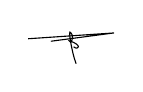
\begin{tikzpicture}[x=1em,y=1em]\draw (-1.6,0.04) -- (1.5,0.25) -- (-0.78,-0.05);\draw (0.13,-0.86) .. controls (-0.02,-0.48) and (-0.17,0.42) .. (-0.07,0.27) .. controls (0.1,0.09) and (-0.09,-0.19) .. (-0.11,-0.04) .. controls (0.38,-0.18) and (0.21,-0.40) .. (0.04,-0.25);\end{tikzpicture}}

Supposons maintenant que de plus, nous nous donnions une section $s$ de $X$ \deleted{\unsure{par}} sur $S$, ne rencontrant pas $X'$ (i.e. une section de $X-X'$ sur $S$). Son image par $j$ est alors une section de $P^1_S-(\infty)$\deleted{\unsure{,|0}}, i.e. une section de $\underline{\mathcal O}_S$, \unsure{appelé|appelée} \uline{l'invariant} de $(X,X',\deleted{\unsure{j}}s)$, soit $\deleted{j}i$

Supposons que l'invariant $\deleted{j}i$ ne prenne nulle part les valeurs $0,1$ i.e. soit inversible, ainsi que $\deleted{j}i-1$. Alors \unsure{sché|sch\textsuperscript{é}} image inverse dans $P^1_S$\deleted{$\unsure{X}$} de $p:S\to P^1_S$ définit un \deleted{section} \inserted{revêt\textsuperscript{mt}} \uline{galoisien} \uline{de} $S$, \uline{non ramifié}, \uline{de groupe} $\mathfrak S_3$, \deleted{\unsure{ici}} \uline{et c'est celui qui définit} $X$. [À \unsure{déduire les fonct\textsuperscript{is}|décrire les fonct\textsuperscript{is}|discuter les problèmes}
% archive sheet number: 43
